\documentclass[10pt,a4paper,notitlepage, twocolumn]{article}
\usepackage[utf8]{inputenc}
\usepackage{amsmath}
\usepackage{amsfonts}
\usepackage{graphicx}
\usepackage{amssymb}
\usepackage{float}
\usepackage{listings}
\usepackage{lipsum}

\author{Nathaniel Forde}
\title{Decision and Expected Value}
\begin{document}


\section*{Expectations: The Workhorse}
There is an algorithm beloved by bureaucrats, the unsung hero of administrators and accountants. An algorithm  both ubiquitous and under appreciated. It's pivotal for nearly every project and informs the actions of tech giants and policy makers the world over. It is only mildly hyperbolic to say that understanding this formula unlocks wealth and power. It lies at the heart of online A/B testing, all policy analysis, sound business strategy and poker play. In words: The expected financial value of a random process is just the sum of the evaluated outcomes weighted by their probabilities. 
$$ EV(O)_{p} = p_{1}v(o_{1}) + p_{2}v(o_{2}) + ... + p_{k}v(o_{k}) $$
Outcomes can vary from deals of cards, to customer transactions and election results. \footnote{In the jargon $O$ is a random variable which can be realised as any of the outcomes  $ o_{j} :  1 \leq j \leq k$} But aside from the mercenary possibilities, Pascal argued such considerations could compel belief in God. The formula, I'd argue, merits your attention for more mundane reasons too. With real stakes on the line, the meaning of probability is not an idle concern. The formula for expected value is glossed as one which governs rational action - surely you want maximise your expected value? Yet, statistics are often tortured to rubber stamp decisions and probabilities are abused to fit policy prescriptions. False precision of risk models is common place, often callous, and occasionally insidious. Yet the crisp clarity of the rule has an enduring appeal that promises to clear the murky waters of probability.

\subsection*{Two sides of a Coin}
Probability has a dual aspect. On one reading it refers to the long run tendency of a random process, on another the probability is construed as the degree of belief in the an outcome. On the first (frequentist) interpretation a probability distribution has certain fixed theoretical characteristics, as in a uniform probability distribution of a fair coin where all outcomes are equally likely. On the second (Bayesian) reading the characteristics of the probability distribution are learned from the data. These approaches are united by the Law of Large numbers which states that as the size of our sample increases our sample average will converge to the expected realisation of the theoretical process.
$$  \frac{1}{N} \sum_{i = 1}^{N} O_{i} \text{ converges to }  E(O) \text{ as } N \text{ approaches } \infty $$ 
In the below plot we have stipulated a Poisson distribution with a mean of 4.5 and can see three examples of how consecutive averaging from the increasing sample sizes results in a closer and closer convergence to the population mean.

\begin{figure}[H]
  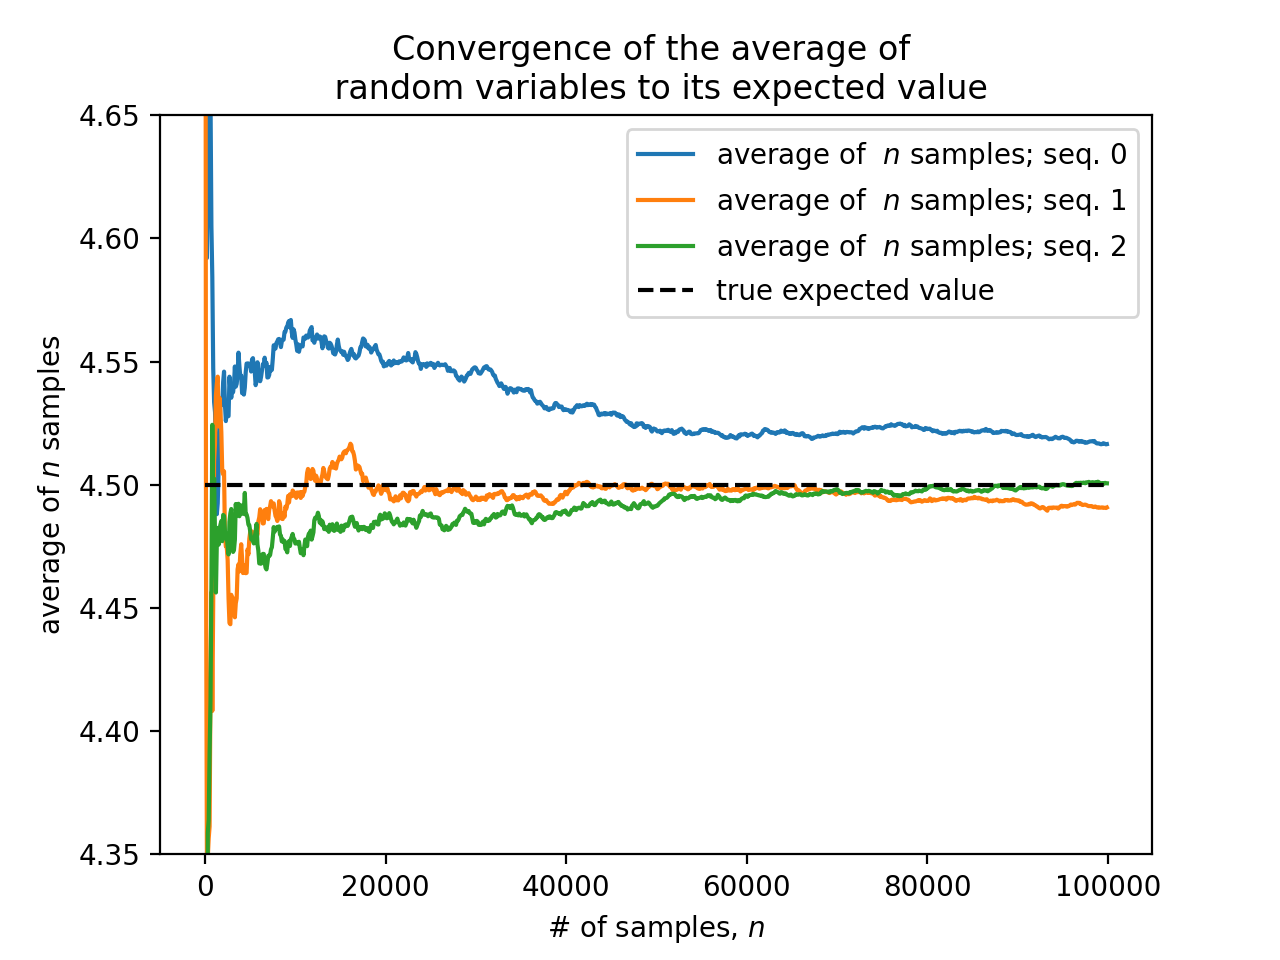
\includegraphics[width=\linewidth]{./Plots/convergence_of_law_of_large_numbers.png}
  \caption{Convergence with large samples}
\end{figure}
\noindent  This is fundamental to the interpretation of probability. Given a game with fixed and fair odds we see that repeated play will converge because of characteristics which govern the process. Dice are the paradigm example.  In the wild we never know the characteristics which cause the observed spread of outcomes, but such is the influence of gambling on the consideration of probability, that by default we assume a stable pattern in the generating process. Partially this is pragmatic. The maths are more tractable if we can assume one well behaved underlying process. The results are compelling. The Normal (Bell Curve) distribution, the Poisson distribution the Bernoulli distribution (to name a few) are all rightly famous. Their shapes are characteristics of innumerable random processes. But the paradigm clouds the fact that in practice we start on the left side of the law of large numbers (with samples) and we often start with small numbers. 
\begin{figure}[H]
  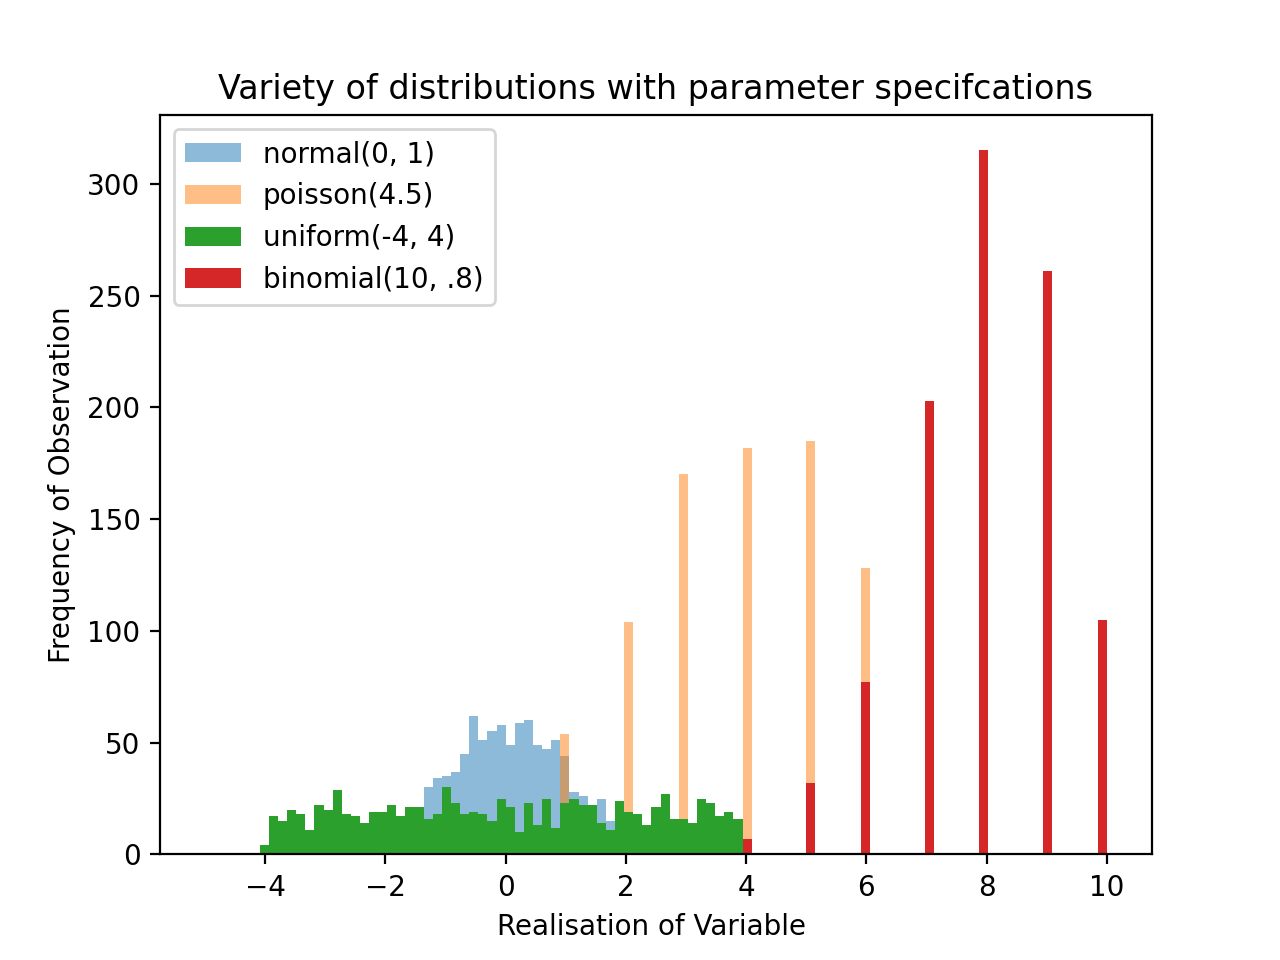
\includegraphics[width=\linewidth]{./Plots/variety_of_distributions.png}
  \caption{Some theoretical distributions with parameters}
\end{figure}
Well behaved probability distributions are rare beasts; a tiny fraction of the world's arbitrary menagerie. The fundamental question in probability is not whether probability is a measure of belief or frequency - it is whether we can safely assume that the underlying process adheres to a known model? If so, we can rely on the structure of the model's theoretical distribution to inform inference. If not we are better learning from the data - trusting to the sampling distribution and worst scenario planning. The challenge is knowing which scenario we're in.

\subsubsection*{Models, Errors and Expectations}
When your only tool is a hammer, then everything is a nail. When one model won't do, use two. This is roughly the approach adopted when models fail. The problem is especially vivid in forecasting; projected death rates, body counts and stock prices are all subject to sudden shocks. A basic regression model tries to predict an outcome $Y$ as linear function of $X$:

$$ Y = const + \beta X + \epsilon $$

\noindent where $\epsilon$ is a random variable representing the error (or noise). A modest notational device for disaster. While $const, \beta$ are parameters estimated by an optimisation process to ensure the equation fits the data as neatly as possible. In the below graph we have a series characterised by change. After the first shock we can refit the model so that the line tracks well with the evolving data. After the second shock we try another refit, but the range the and variance of the data makes our basic model a poor fit i.e. the data no longer exhibits a linear relationship. This presents three examples of error in the modelling process: (i) forecasts fail for the reason that's it's also difficult to identify (in the moment) those changepoints in the data which reflect structural change, (ii)  the fundamental assumptions that go into the model are sound, but the parameters need be re-estimated based on the new data
\begin{figure}[H]
  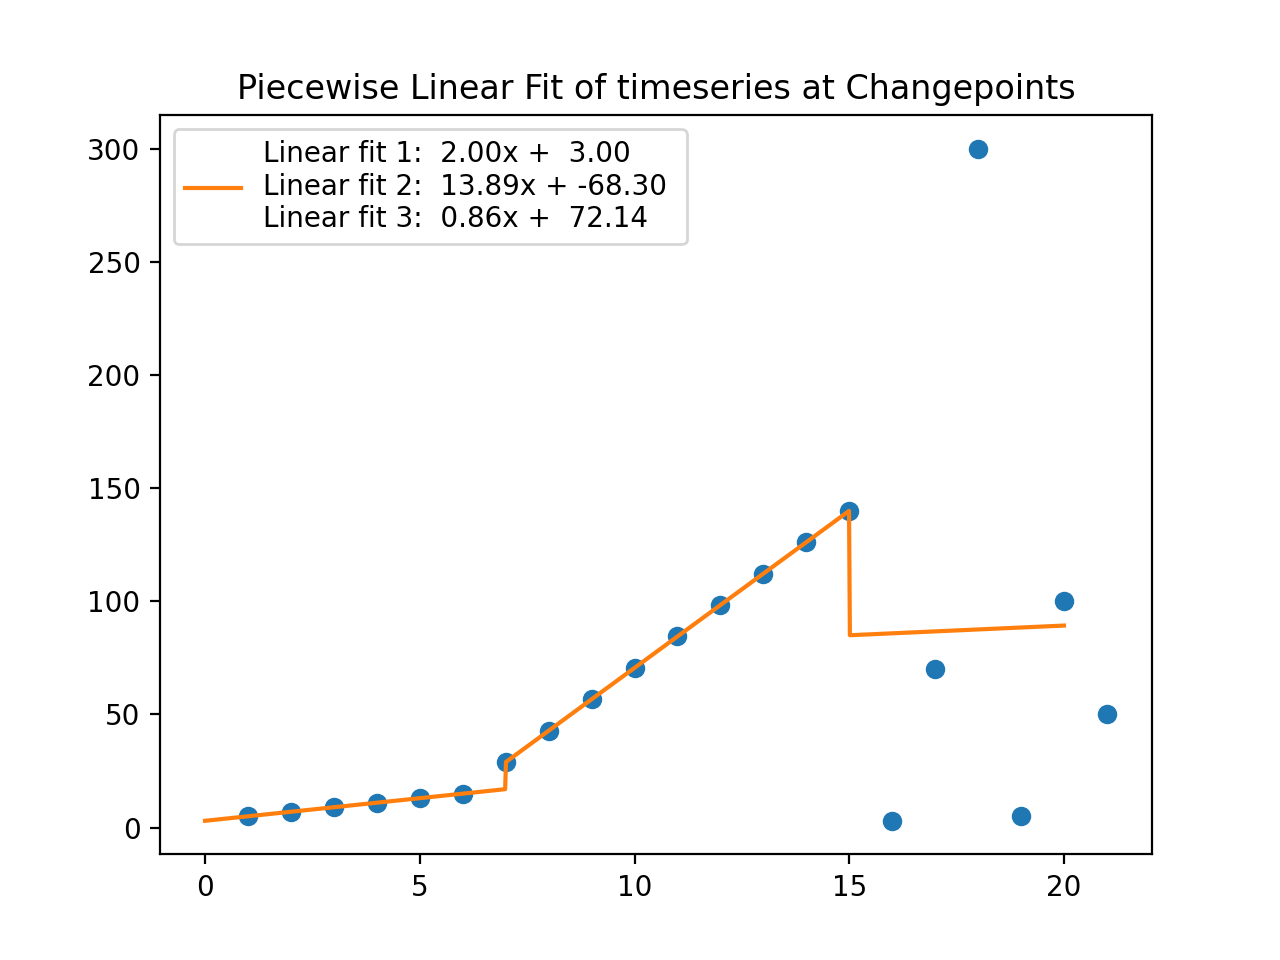
\includegraphics[width=\linewidth]{./Plots/piecewise_linear_fits.png}
  \caption{Three samples with starkly different parametrisations}
\end{figure}
and (iii) the third linear model is simply a terrible match for the pattern in the data. In practice you never really know whether a new error stems from a misfit but appropriate model or an entirely inappropriate model. But as we increase our number of sample fits we hope to better approximate the true linear process (if any) generating the data. This warrants a note about errors. Imagine now that the data points on our previous graph are repeatedly re-speckled over the canvas. We can refit a new model for each set of scattered data points and each refit gives us a new sample values for $ const, \beta$. If the underlying data generating process is stable, then the parameter fits will converge to the correct values of $const, \beta$; correct in the sense that they can be used to draw the line of best fit for the data. A statistically stable process is one that can be modelled with errors $\epsilon$ normally distributed around 0, so that the model will be \textit{ correct on average.} Our predictions will overshoot in some cases but on the whole the errors up and down will cancel each other out. Forecasting with the parameters of best fit minimises our forecast errors because the fluctuations are stable about the centre of the line. These are assumptions required for a process to exhibit the tendency of regression towards the mean. If they're not met, we will see poor parameter estimates and wild swings away from the linear path.
\newline

\noindent The code below builds two sampling distributions based on different underlying processes.  One in which the errors are independent, normally distributed around 0 the other in which the errors are correlated in a sine-wave like pattern, increasing and decreasing periodically. This is akin to difference between measuring error when predicting the heights of randomly sampled people versus predicting the sales volumes on randomly selected days of the week. A random sample of daily sales  risks clumping weekends together and skewing the expected values. No such risk exists when sampling from independent individuals. 

\begin{lstlisting}[language=Python]
### Build True Models
N = 100000
X = np.random.uniform(0, 20, N)
independent_err = 
np.random.normal(0, 10, N)
corr_err = 
np.random.uniform (0, 10) + 
np.sin(np.linspace(0, 10*np.pi, N)) + 
np.sin(np.linspace(0, 5*np.pi, N))**2 + 
np.sin(np.linspace(1, 6*np.pi, N))**2

Y_corr = -2 + 3.5 * X + corr_err

Y = -2 + 3.5 * X + independent_err

population = pd.DataFrame({'X': X,
 'Y': Y, 'Y_corr': Y_corr})

### Sample from Data 
### and build smaller models

fits = DataFrame(columns=['iid_const',
 'iid_beta', 'corr_const', 
 'corr_beta'])
 
for i in range(0, 10000):
    sample = population.sample(n=100, 
    replace=True)
    Y = sample['Y']; X = sample['X']
    Y_corr = sample['Y_corr']
    X = sm.add_constant(X)
    iid_model = sm.OLS(Y, X)
    results = iid_model.fit()
    corr_model = sm.OLS(Y_corr, X)
    results_2 = corr_model.fit()
    row = [results.params[0], 
    results.params[1],
    results_2.params[0], 
    results_2.params[1]]
    fits.loc[len(fits)] = row
    
fits.boxplot()
\end{lstlisting}

\begin{figure}[H]
  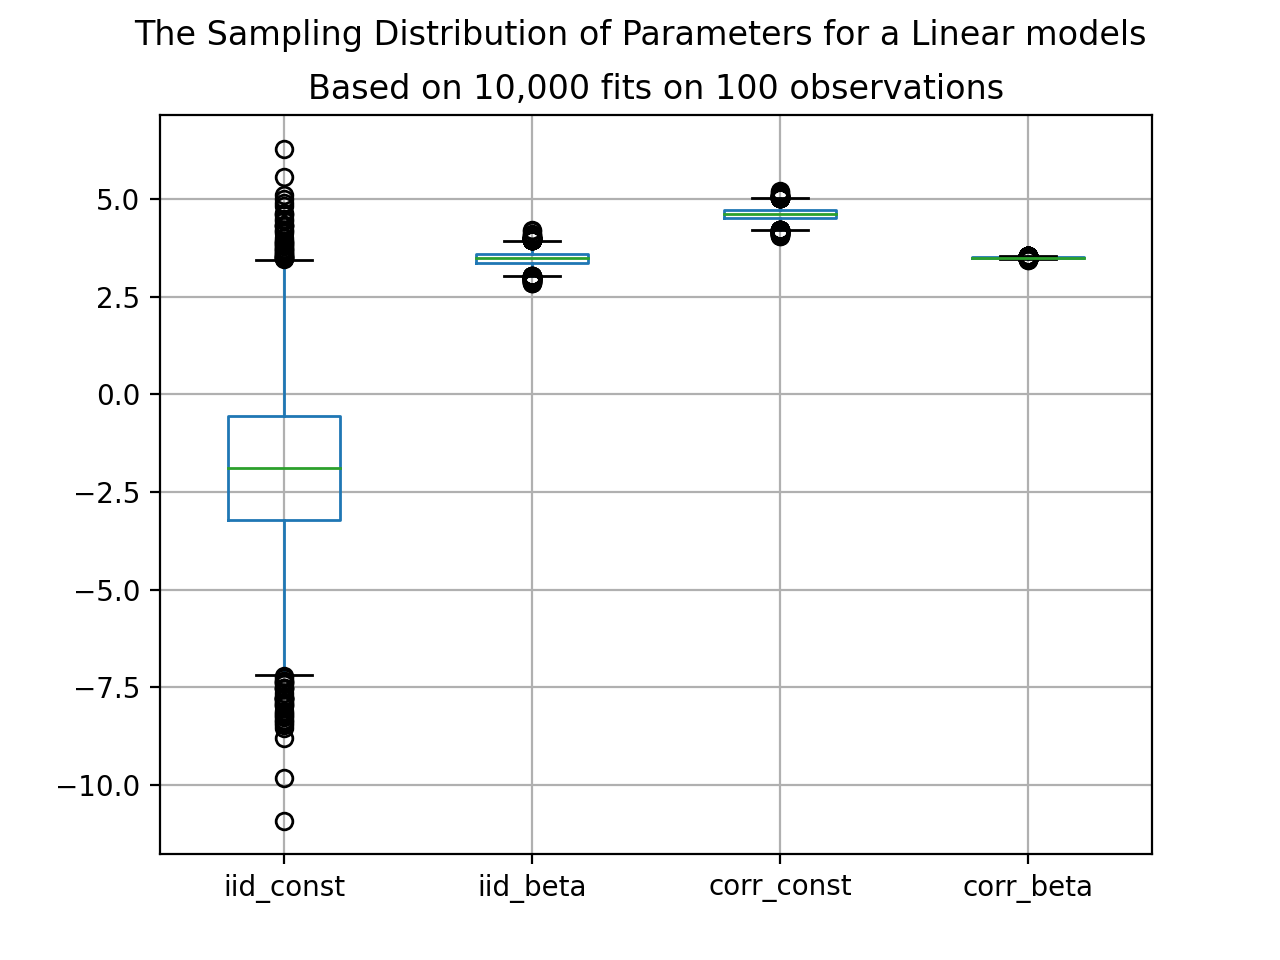
\includegraphics[width=\linewidth]{./Plots/distribution_of_beta1.png}
  \caption{Sample fits for $\beta, const$ with different errors structures}
\end{figure}

In the case with independent errors the expected value for our parameter estimates match almost exactly the true values of the process. In the second model with correlated errors the parameter estimate for our constant is 4.9 which is significantly different from the true value of -2, and will lead to systematically skewed predictions. Statistical models are just algebraic equations where we use regular sampling to solve for $Y$, but the solutions are always approximate, skewed by inadequate or inaccurate data as much as by poor choices in model design. 

\subsection*{Small Worlds, Inference and Decision}
Prediction precedes probability in the order of analysis. Without a reliable regularity underwriting our observations, we interpret them as timorous noise. Only when there is a better than arbitrary correlation between $X, Y$ will we even think to ascribe a measurable probability to their association. Whether we view probabilities as a measure of credibility or frequency, the focus is always on a process which in reality reveals a pattern under repetition. We're loath to apply a probability model of any kind without some base inductive evidence.
\newline 

\noindent So when does it make sense to use models? In what sense should expected values guide our action? If models are mere heuristics, from where do we pluck the values for $$p_{i} : 1 \leq i \leq k$$ in the formula $(EV)$. Models are deliberate simplifications of complexity, toy versions of the world. While recent innovations of in machine learning means that we can fit models with hundreds, thousands and even billions of parameters but this increase in scale does not change fact that models are blind to all factors outside their samples. A good model predicts the variance in future data, in part, by ignoring the genuine complexity of reality. This is the only practical test that matters. If the prediction accuracy holds over successive periods we should become increasingly sure that the probabilities in our model are a good measure of risk. We can't be certain the model holds over all successive periods - robust to changes in external factors. We can however quantify the degree of uncertainty in the model by observing the spread of the sampling distribution. The expected revenue of a process depends on this uncertainty and the finer points of statistical inference. 

\subsubsection*{Inference from Expected Frequency}
If you count the number heads in a series of 5 successive coin flips, you'll arrive a proportion which characterises that process. Repeat the process 1000 times and you'll have something like the true distribution. If it's a fair coin the long run expected result will be half the number of your coin flips. If the coin is weighted you might have as few as 0. This is the binomial distribution, and it really shines when you're trying to gauge fairness. If a process is biased, the distribution will be skewed. We can use this fact for inference. Consider a dispute over whether the game was rigged. 
$$ H_0 : \text{ true proportion of heads } = 0.4  $$
$$ H_1 : \text{ true proportion of heads } =  0.5 $$

\noindent Take $(H0)$ as given then if we observe a sequence: $$ (3in5): H, H, H, T, T$$, what does this say about the possibility that we're being hustled? If the coin is biased, then the count of heads in repeated sampling will reflect a clear bias. For any new data we can check if the data is consistent with the data generated by the biased coin. The pattern of reasoning is straightforward (i) make some assumptions about the structure of the random process under investigation, (ii) tease out the consequences of these assumptions (iii) evaluate the incoming data against these consequences to see if you need to revise your assumptions. Is the data weird given the assumed shape of our probability distribution?

\begin{figure}[H]
  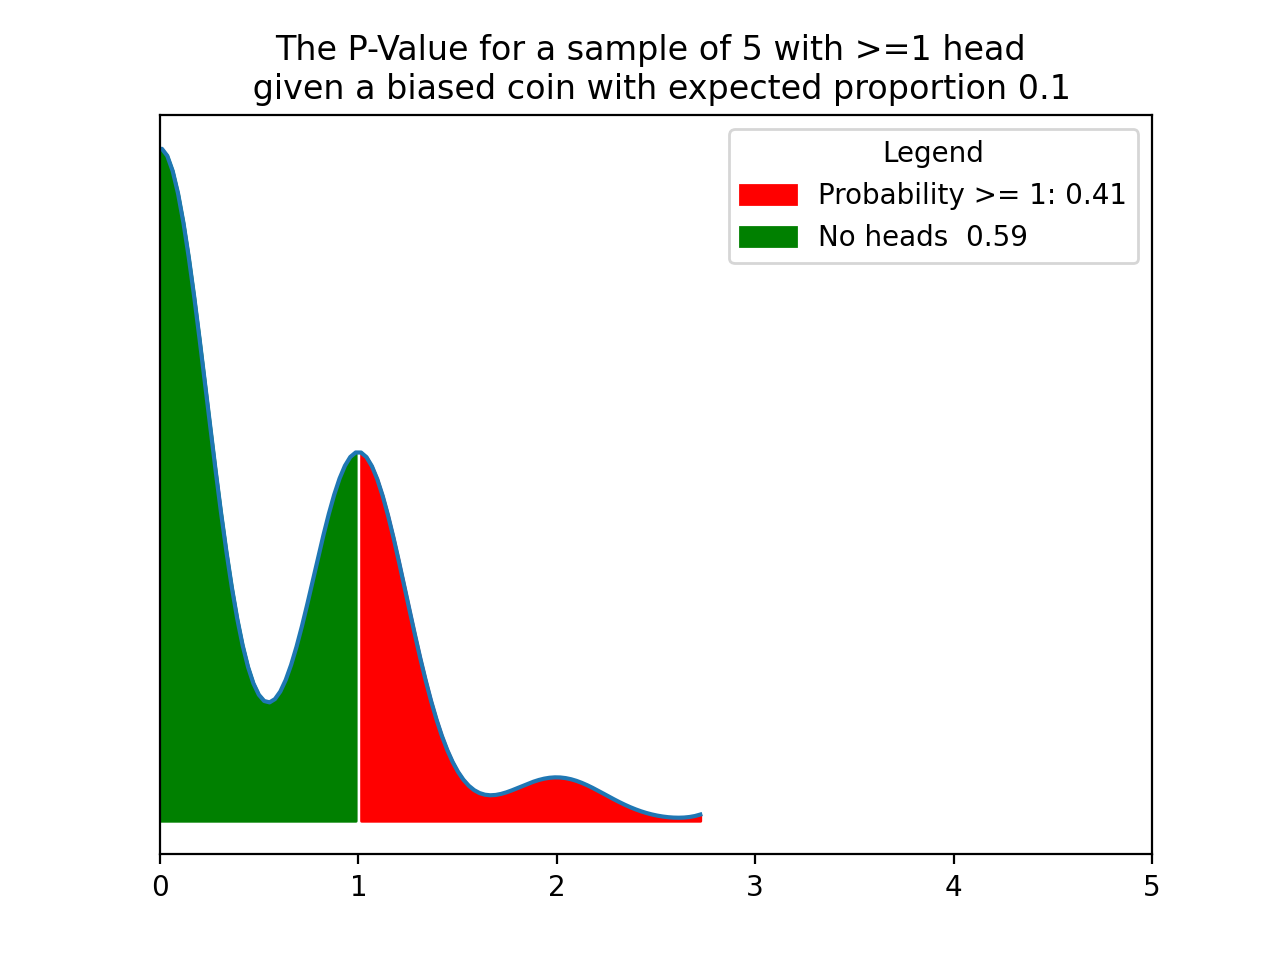
\includegraphics[width=\linewidth]{./Plots/binomial_test.png}
  \caption{The Binomial Distribution}
\end{figure}

In this instance the shape of the binomial distribution defined by a 0.4 biased coin allows for significantly greater than  5\% chance for observing the above sequence. So we do not have enough reason to reject $(H0)$ at the traditional threshold. By design the assumed distribution builds in characteristics of long-run variance of the process, and the slim threshold for rejection is designed to minimise errors. Without enough observations the sample distribution is unlikely to be properly centred around a stable point. This makes even small p-value thresholds unreliable. Elections are an example of repeated process which (arguably) offer a repeated choice, but political dynamics are such to undermine the statistical properties of an apparent binary choice. One voter is not easily exchangeable with another, a sample poll in Texas is not the same as one in New York. We cannot blindly take a sample poll to imply the spread or volatility of a population, and with low samples it's hard to justify any kind of inference from expectation.

\subsubsection*{Inference from Prior Belief}
On the other hand if we instead use probability to calibrate our beliefs, then we should be more explicit in our assessment of $(H0), (H1)$. Let's assume that our prior beliefs about whether the game is rigged is 50/50. Then we evaluate the two hypothesis using Bayes's rule for incorporating our prior belief and the data. 

$$ \overset{posterior}{p(H_{i} | Data)} = \frac{\overset{prior}{p(H_{i})}\overset{liklihood}{p(Data | H_{i})}}{\underset{evidence}{\sum_{i=1}^{i =K} p(Data | H_{i})p(H_i)}}$$

where $ 1 \leq i \leq K$ spans the ways in which the data could have been realised. Then we have:

$$ \frac{p(H_1 | 3 in 5)}{p(H_{0} | 3 in 5)} = \frac{\frac{.5\cdot .23}{.5\cdot .32 + .5 \cdot .23}}{\frac{.5\cdot .32}{.5\cdot .32 + .5 \cdot .23}} = \frac{.57}{.42} $$

which would lead us to infer that the coin was fair. Note that the example slightly obscures the difference between Bayesian and frequentist methods. since we're considering gambling odds we want our beliefs to reflect the long run odds and the disagreement appears only in so far as we've allowed for our priors to influence the outcome. However the really radical move in the Bayesian setting is that you're allowed to ascribe a probability to any event regardless of whether there is any long-run sequence to observe. You may know nothing about your opponent or the coin, but for Bayesians this is no bar to assigning suspicion in the form of expected probability ,so long as you act in accordance with the axioms of probability. It's this freedom which can seem arbitrary and unmotivated, but in practice probabilities  are rarely ascribed without reason.

\raggedbottom

\subsection*{Big Data and Expected Returns}
Neither style of analysis ends with these calculations, both would continue to probe the limits of each hypothesis. We'd have to consider things like sample size and sensitivity testing, model performance and cost of errors. The point is just that there are reasons for dispute. This example shows the heart of the conflict in the dual aspect of probability. There is enough latitude in the manner in which we set up a probability model that the mathematics can yield apparently inconsistent results. The frequentist evaluation of our biased coin is very sensitive to the choice of hypotheses, while the Bayesian approach is influenced by the choice of prior. Why set up a significance test against assumed cheating rather than assumed fairness? Why attribute equal weight to both hypotheses? Why use a 5\% threshold if you're concerned about systematic cheating? Both offer strategies for managing uncertainty, but both approaches come with baggage, that not even Big data can solve.
\newline 

\noindent What is Big Data? Does it solve anything? There is some hype over the term, but it's not magic it's just bigger sample sizes for niche questions. Websites and apps collect traffic and log interactions. Your details are captured and pulled into vast aggregates of consumer data. I can route and re-route your trajectory across an online environment. Applying the same pressures to tens of thousands of others, we can trace out how the topology of particular sites throw up speed bumps on the customer's journey. 
Imagine we're running a website which aims to funnel customers through to a number of different purchase plans. The historic patterns are relatively stable with only 10\% of customers dropping out of our conversion funnel on a daily basis. We can sample actions online under differing pressures with a view to evaluating expected values of repeated coercive prompts.

\begin{figure}[H]
  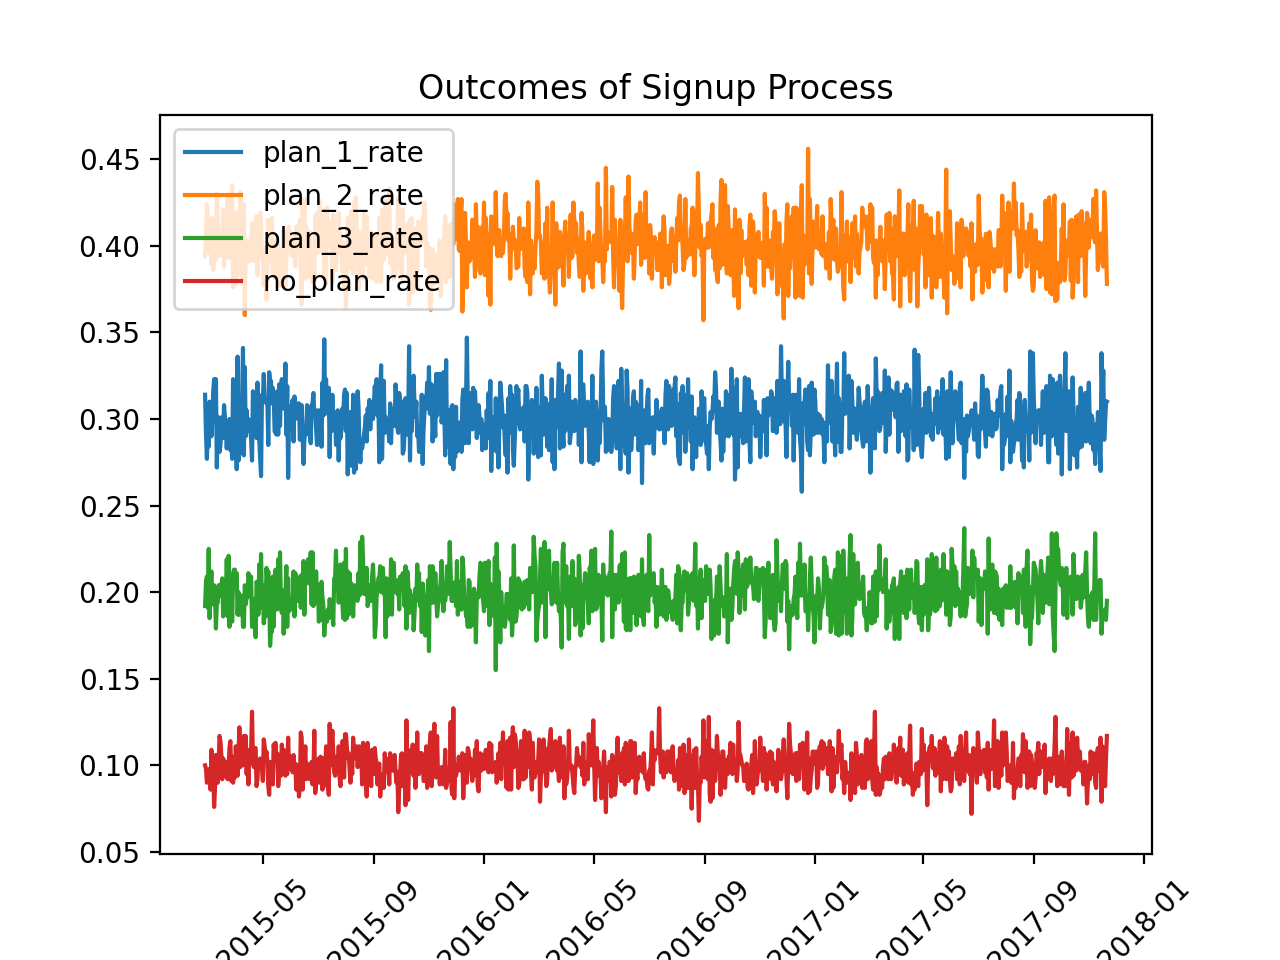
\includegraphics[width=\linewidth]{./Plots/outcomes_of_signup.png}
  \caption{Stable long run Sign Ups }
\end{figure}

Assume the particular values for each plan then the expected value of customer journey is just: $ p_{1}v(o_{1}) + p_{2}v(o_{2}) + p_{3}v(o_{3}) + p_{4}v(o_{4})  = .3*10 + .4*7  + .2*12 + .1*0 = 8.20.$ Now imagine there was a change to the website and we observe the following pattern for the next 20 days:

\begin{figure}[H]
  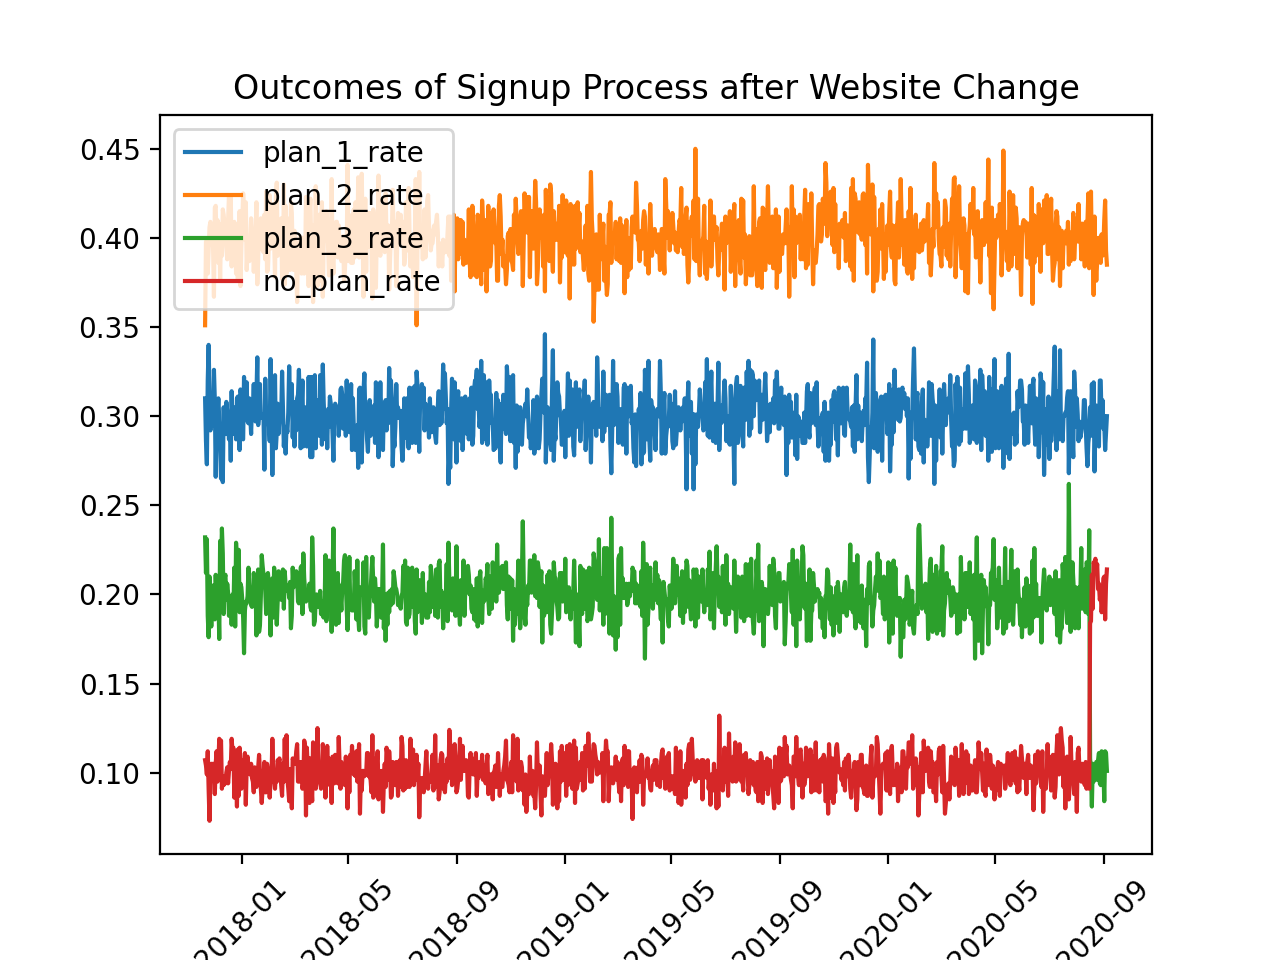
\includegraphics[width=\linewidth]{./Plots/outcomes_of_signup_post.png}
  \caption{Abrupt increase in dropouts}
\end{figure}

What is the new expected value? From the frequentist point of view the macro distributional properties haven't significantly changed. But given what we know about the change to the website it would be foolish to assume such a static distributional assumption. Looking only at the small sample of new data, the variance will be large and the estimates of rates of signup for each plan will be unstable.  Following the Bayesian paradigm we can condition on our expectations on the new data, the old data or all the data we get slightly different results. 

\begin{figure}[H]
  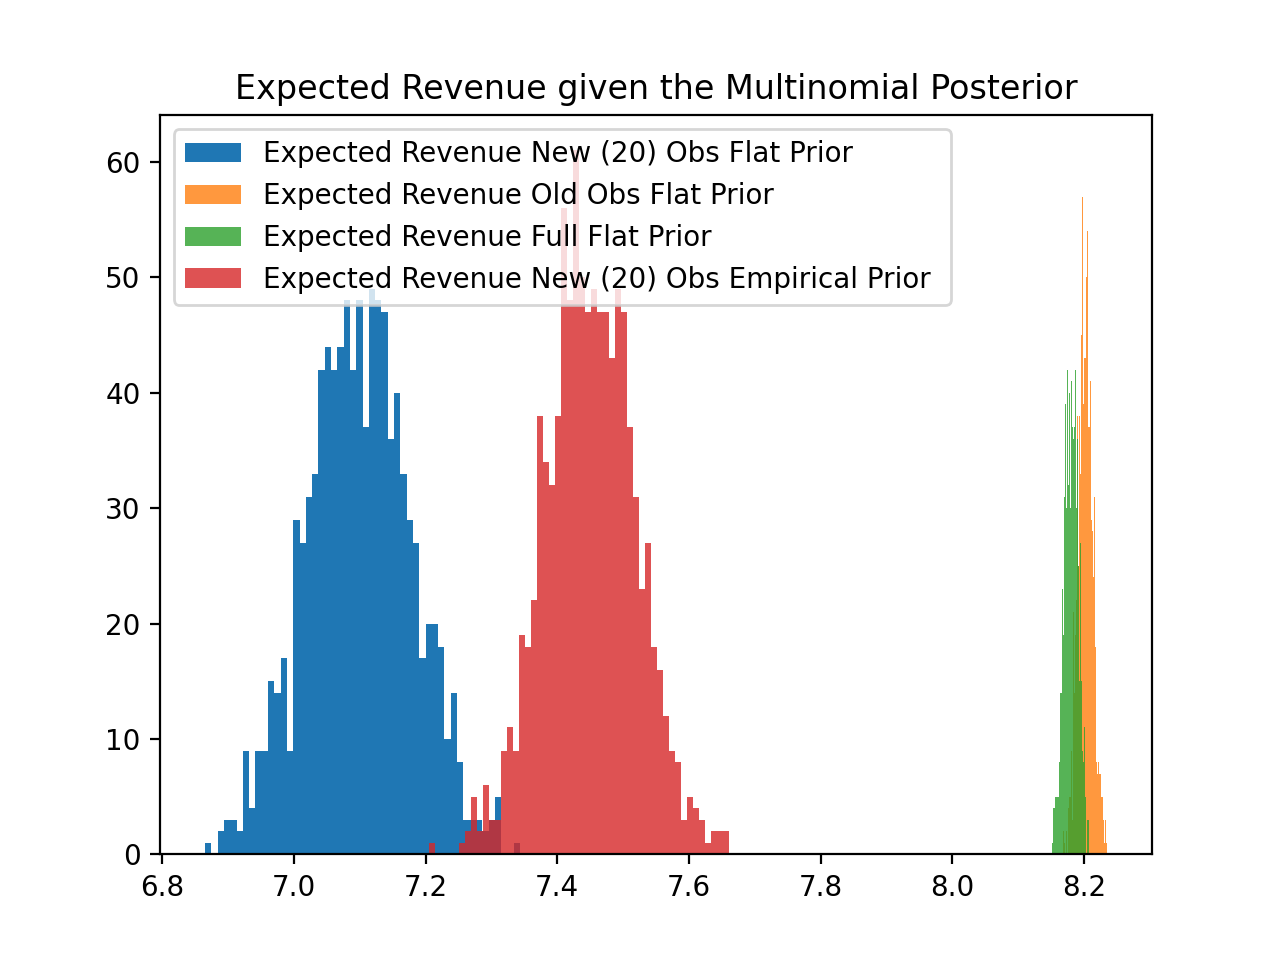
\includegraphics[width=\linewidth]{./Plots/expected_revenue_distributions.png}
  \caption{Expected revenue differs by choice of prior and data to conditionalise}
\end{figure}

Using a large number of observations, the influence of our priors are minimal and washed out by the data, giving us a strong point estimate with low variance stable around 8, but since the recent data involves a step change, we might be better off ignoring the old data. But we can also see that if we condition our expectations only on the new data with different priors drawn from the past data or hope, we can positively bias our expectations. The point here is that nearly all substantial decisions are made with small samples in circumstances where past behaviour is not a guide. More to the point, past behavioural patterns are exactly what we're trying to avoid or change. If you want to know whether the change on your website will drive a material change in financial revenue, you won't have long run patterns to rely on and it's an open question on how to weight the new data. 

\subsection*{Wither Expectation?}

\end{document}

